\documentclass[]{book}
\usepackage[english]{babel}
\usepackage{graphicx}
\usepackage{amsmath}


\begin{document}
\chapter*{Overview on GEM Detectors}

En numerosos experimentos de física de partículas, los detectores gaseosos, incluidos los GEMs, desempeñan un papel crucial en la medición de partículas cargadas mediante la ionización de gases. Estos detectores permiten trazar con precisión las trayectorias de las partículas, especialmente en entornos con campos magnéticos. En comparación con los detectores de semiconductores, los detectores gaseosos suelen ser más económicos, especialmente en aplicaciones que requieren cubrir grandes volúmenes, y presentan menos material que pueda interferir con las partículas que atraviesan el detector [1]. Dado que los detectores GEM son el enfoque principal de este trabajo, en el presente capítulo se explorarán los conceptos fundamentales de la física que rigen sus interacciones y funcionamiento.

\section{Electromagnetic interactions of charged particles with matter}

\noindent De manera general, el proceso de detección de una partícula cargada es posible gracias a la deposición de una fracción o toda su energía en el medio con el cual interactúa. Si bien es posible observar fenómenos como la luminiscencia, centelleo o ionización como resultado de la interación entre partículas cargadas y medios gaseosos, la interacción prevalente en sistemas de baja densidad que puede ser explotada para extraer una señal medible es la ionización.\\

\noindent Si los fenómenos de ionización en un gas son estudiados de manera independiente en este contexto, es posible realizar una descripción que sigue la estadística de Poisson

\begin{equation}
    \label{eq:poisson}
    P_k^n=\frac{n^k}{k!} \mathrm{e}^{-n}
\end{equation}

\noindent La eficiencia teórica del detector, definida como la probabilidad de tener al menos una interacción, es entonces

\begin{equation}
    \label{eq:det_eff}
    \varepsilon=1-P_0^n=1-\mathrm{e}^{-n} .
\end{equation}

\noindent No existe una expresión simple para determinar el número de encuentros ionizantes primarios; por lo tanto, es necesario recurrir a datos obtenidos experimentalmente o a programas de simulación especializados. Si no se tienen en cuenta procesos secundarios como la recombinación, por ejemplo, siendo $\Delta E$ la energía depositada en el medio y $W_{I}$ la energía por par íonico, la cantidad total de pares iónicos en el medio puede ser calculada como 
\begin{equation}
    \label{eq:num_ion}
    N_{T} = \frac{\Delta E}{W_{I}}.
\end{equation}

No obstante, este es un resultado promedio. Para entender con detalle la distribución energética en este fenómeno, es necesario acudir a un marco teórico más robusto.

\subsubsection{Stopping-power}

\noindent La pérdida de energía cinética de la partícula a medida que avanza por el volumen del detector es conocida como stopping power o ecuación de Bethe-Bloch. Una formulación semiclásica para calcular la energía liberada por la partícula al atravesar un medio de grosor $\Delta x$ es: 

\begin{equation}
    \label{eq:bethe_bloch}
    \frac{\Delta E}{\Delta x}=-\rho \frac{2 K Z}{A \beta^2}\left[\ln \frac{2 m c^2 \beta^2}{I\left(1-\beta^2\right)}-\beta^2-\frac{C}{Z}-\frac{\delta}{2}\right], \quad K = \frac{2 \pi N e^{4}}{mc^{2}}
    \end{equation}

donde $\beta$ es la velocidad de la partícula, $m$ y $e$ son la masa y la carga del electrón, $Z$, $A$ y $\rho$ son el número atómico, masa atómica y la densidad del medio, $I$ es el potencial promedio de ionización del medio, el término $C/Z$ hace referencia a correcciones por apantallamiento con capas electrónicas internas y $\delta /2$ solo tiene relevancia en el régimen relativista. Para estimar las mencionadas correcciones, es necesario acudir a tablas de referencia o hallar los parámetros a partir de ajustes con datos experimentales.\\ 

\noindent Algunas consideraciones que deben ser tenidas en cuenta respecto a la ecuación de Bethe-Bloch, son su aplicabilidad a medios isotrópicos, debido a la aparición de "channeling effects" en sistemas cristalinos y las excepción de electrones y protones como partículas incidentes por su indistinguibilidad en la materia [2].\\

\noindent Teniendo en cuenta que la velocidad de la partícula ionizante es uno de los parámetros que rigue la ecuación \ref{eq:bethe_bloch}, es posible describir el comportamiento de su pérdida de energía para distintos regímenes de velocidad. Como ilustra la figura \ref{fig:bethe_b} [3].

\begin{figure}[h]
    \centering
    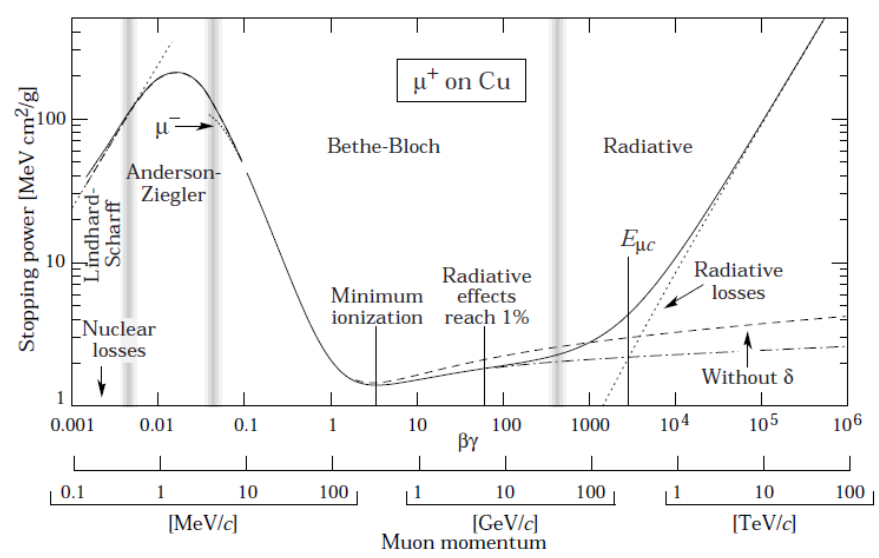
\includegraphics[width=0.8\textwidth]{bethe_bloch.PNG}
    \caption{La fórmula de Bethe-Bloch para muones positivos en cobre como función de la velocidad [3] (mostrada entre la segunda y tercera banda gris. El resto se describe mediante otros modelos).}
    \label{fig:bethe_b}

\end{figure}

\section{Gaseous detectors}

\noindent La base para la detección de partículas en los detectores gaseosos es la creación de cargas mediante ionización. Para la eficiencia en la formación de señales, también es crucial que las cargas no se pierdan por recombinación o adherencia mientras se desplazan hacia los electrodos.

\section{GEM detectors}

\subsection*{References}
\begin{enumerate}
    \item Sauli, F. (2015). Gaseous radiation detectors: fundamentals and applications (p. 497). Cambridge University Press.
    \item Giovani Mocellin. “Performance of the GE1/1 detectors for the upgrade of the
    CMS Muon Forward system”. PhD thesis. Rheinish-Westf¨alische Technische
    Hochschule Aachen University, 2021. url: https://cds.cern.ch/record/
    2809098.
    \item K Nakamura and (Particle Data Group) 2010 J. Phys. G: Nucl. Part. Phys. 37 075021. DOI 10.1088/0954-3899/37/7A/075021
\end{enumerate}

\end{document}